%----------------------------------------------------------------------------------------
%	PACKAGES AND OTHER DOCUMENT CONFIGURATIONS
%----------------------------------------------------------------------------------------

\documentclass{article}

\usepackage{lastpage} % Required to determine the last page for the footer
\usepackage{extramarks} % Required for headers and footers
\usepackage{graphicx} % Required to insert images
\usepackage{gensymb}
\usepackage{hyperref}

\linespread{1.1} % Line spacing
\usepackage[total={6in, 9in}]{geometry}

\setlength\parindent{0pt} % Removes all indentation from paragraphs



\begin{document}
\title{Advanced Computer Graphics\\ Coursework 2}
\author{Terence Tse, Zhou Yu \\ Team JT}
\maketitle
\newpage

\section{Part 1: Fresnel reflectance}
Using the equations outlined in the notes for Fresnel reflectance,
the graph depicting parallel and perpendicular components of air to glass
(or some other material with a refraction index of 1.5)
which was a refraction index of $1.0$ to $1.5$ and can be seen in Figure 1. The
graph of Fresnel Reflectance from glass to air ($1.5$ to 1.0) is shown in 
Figure 2. The curve for Schlick's approximation of Fresnel
reflectance is seen in Figure 3. These can all be found in the ``part1" folder
in the pictures folder of the attached files.\\
\\
From air to glass, we took the parallel component measurements and found
Brewster's angle to be \texttt{0.9837 radians}  ($56.3636\degree$).

\begin{figure}[h]
	\centering
	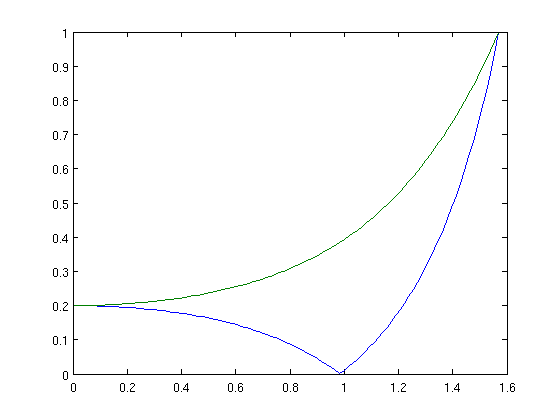
\includegraphics[scale=0.5]{pics/part1/air2glass.png}
	\caption{From a 1.0 index of refraction to 1.5.
				The x axis shows the angle in radians that 
				light hits the second material. The Y axis
				shows the fresnel reflectance.}
\end{figure}

From glass to air, we took the parallel component measurements and from here
could owrk out the critical angle to be \texttt{0.7299 radians} 
($41.8182\degree$).

\begin{figure}[h]
	\centering
	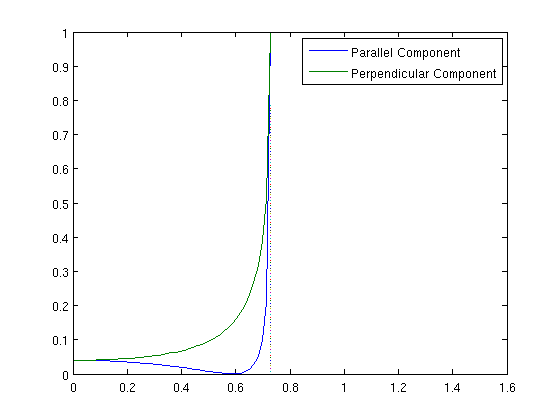
\includegraphics[scale=0.5]{pics/part1/glass2air.png}
	\caption{From a 1.5 index of refraction to 1.0}
\end{figure}

\newpage

Finally, with Schlick's approximation, we made sure to use the reflectance
of normal incidence from the air to glass Fresnel reflectance graph which 
was $0.04$ from ($0.2^{2}$).

\begin{figure}[h]
	\centering	
	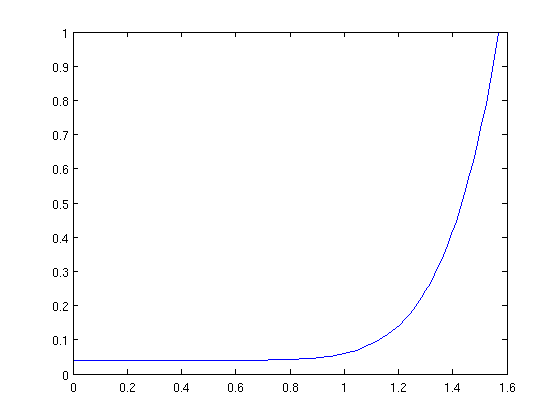
\includegraphics[scale=0.5]{pics/part1/Schlick.png}
	\caption{From a 1.0 index of refraction to 1.5}
\end{figure}


\section{Part 2: Environment Map(EM) sample generation}
The samples we took from the environment map can be see in 
``pics/part2/sample*.pfm" and ``pics/part2/sample*.ppm" in the 
attached files. For each sample pixel, we have surrounded it with a $9$ pixel 
neighbourhood for better visualisation. \\
\\
We have performed sampling with $64$, $256$
and $1024$. The steps we followed were approximately the same as discussed in the
lectures. First we calculated the average luminance of each row of the environment
map, stored them in an array. Then we normalised the array so that the sum of the 
terms will add up to $1$. After we made a cumulative sum of the array so it will 
serve as a cumulative density function. This is done in the very similar manner
on each row.\\
\\
To sample, we then generated two random variables $u$ and $v$ between $0$ and $1$.
We have to first find out which row $u$ is coming from, in other words, the first
index from the luminance array that is greater than $u$. We noticed that since
array is a cumulative density function, it is a increasing array. As a result we  
devised a binary search algorithm to find the index quickly. Similarly, this 
technique can be done on when locating which column $v$ is coming from.\\
\\
This method is faster than the usual linear search on the array, since the complexity
is \texttt{log} in terms of the array size and the other method takes up to 
linear time.

\section{Part 3: Environment Map(EM) Sphere Rendering}
As discussed before in lectures, office sessions and the email, we implemented the Sphere
rendering following Monte Carlo importance sampling.

$$\int L_{i}(\omega i) d\omega i = \frac{2\pi^{2}}{W*H} *\sum_{W*H}L_{i}(\omega i) sin\theta$$

Of course, after this we had to apply another multiplication
by $\frac{1}{\pi}$ due to having a perfectly diffuse BRDF (albedo 1.0). 
From here, we generated our pictures, each time
taking a new set of samples and fixing those samples for the 
current sphere being produced. These pictures can be viewed,
again, in our ``pics" folder, underneath ``part3" where we have
sampled with $64$, $256$ and $1024$ samples: 
``renderSphere64.pfm and .ppm", ``renderSphere256.pfm and .ppm" 
and ``renderSphere1024.pfm and .ppm". \\
\\
As expected, the amount of bias
was seen to decrease, in the 64 sphere, there is little amount of 
orange light which would come from the altar in the scene. This was
most likely due to the sampling not picking enough points from that part of
the Environment map. In the higher sample spheres, we see more contribution
from the altar light.\\
\\
In our pictures, we do observe some strange blue and magenta striping on the
sphere. We assume this is attirbuted to not clamping the terms after computing
the dot product of the sample vector and the pixel normal vector. Some of the
colour channels became negative and we think that HDR shop might be taking the
absolute values of these rather than clamping the contribution to $0$. We did
attempt to clamp any of these negative contributions as light should add intensity
and not remove, even if it adds 0. This resulted in our sphere looking very good in
terms of colour but very flat, like a circle. This can be seen in ``renderNoClamp64.pfm".
\section{Part 4: Rendering a Sphere with Grace EM and PBRT}
Albedo was set at $1.0$ and the three sphere can be seen in the
``part4" folder of the ``pics" folder attached. These are the
.pfm and .ppm images named ``simplesphere8", 
``simplesphere16" and ``simplesphere32" for the $8$, $16$, and
$32$ sample sampling methods.
As we can see from these images the general amount of noise 
decreased quite noticeably from $8$ to $16$ samples and again 
decreased from $16$ to $32$ but less noticeably.

\end{document}
